

\tikzset{every picture/.style={line width=0.75pt}} %set default line width to 0.75pt        

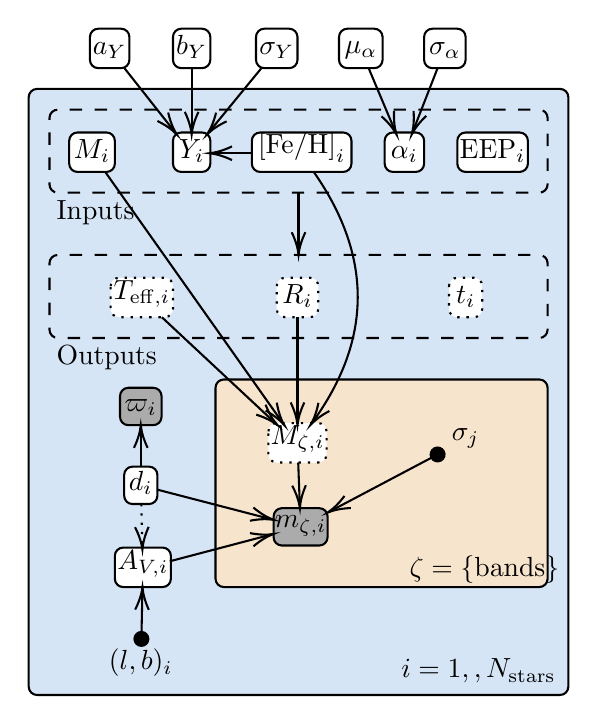
\begin{tikzpicture}[x=0.75pt,y=0.75pt,yscale=-1,xscale=1]
%uncomment if require: \path (0,384); %set diagram left start at 0, and has height of 384

%Shape: Rectangle [id:dp010165550931289014] 
\draw   (50,70) -- (70,70) -- (70,90) -- (50,90) -- cycle ;
%Shape: Rectangle [id:dp9376205267267221] 
\draw  [fill={rgb, 255:red, 214; green, 229; blue, 246 }  ,fill opacity=1 ] (30,54) .. controls (30,51.79) and (31.79,50) .. (34,50) -- (286,50) .. controls (288.21,50) and (290,51.79) .. (290,54) -- (290,338) .. controls (290,340.21) and (288.21,342) .. (286,342) -- (34,342) .. controls (31.79,342) and (30,340.21) .. (30,338) -- cycle ;
%Shape: Rectangle [id:dp0879962430090866] 
\draw  [dash pattern={on 4.5pt off 4.5pt}] (40,134) .. controls (40,131.79) and (41.79,130) .. (44,130) -- (276,130) .. controls (278.21,130) and (280,131.79) .. (280,134) -- (280,166) .. controls (280,168.21) and (278.21,170) .. (276,170) -- (44,170) .. controls (41.79,170) and (40,168.21) .. (40,166) -- cycle ;
%Shape: Rectangle [id:dp4207868301071993] 
\draw   (150,210) -- (170,210) -- (170,230) -- (150,230) -- cycle ;
%Shape: Rectangle [id:dp10030238688422877] 
\draw   (150,250) -- (170,250) -- (170,270) -- (150,270) -- cycle ;
%Shape: Rectangle [id:dp8355634642427261] 
\draw   (230,230) -- (250,230) -- (250,250) -- (230,250) -- cycle ;
%Shape: Rectangle [id:dp5906205088171197] 
\draw  [fill={rgb, 255:red, 246; green, 228; blue, 205 }  ,fill opacity=1 ] (120,194) .. controls (120,191.79) and (121.79,190) .. (124,190) -- (276,190) .. controls (278.21,190) and (280,191.79) .. (280,194) -- (280,286) .. controls (280,288.21) and (278.21,290) .. (276,290) -- (124,290) .. controls (121.79,290) and (120,288.21) .. (120,286) -- cycle ;
%Straight Lines [id:da4973220211869567] 
\draw    (160,100) -- (160,128) ;
\draw [shift={(160,130)}, rotate = 270] [color={rgb, 255:red, 0; green, 0; blue, 0 }  ][line width=0.75]    (10.93,-3.29) .. controls (6.95,-1.4) and (3.31,-0.3) .. (0,0) .. controls (3.31,0.3) and (6.95,1.4) .. (10.93,3.29)   ;
%Shape: Rectangle [id:dp5690927935939454] 
\draw  [dash pattern={on 4.5pt off 4.5pt}] (40,64) .. controls (40,61.79) and (41.79,60) .. (44,60) -- (276,60) .. controls (278.21,60) and (280,61.79) .. (280,64) -- (280,96) .. controls (280,98.21) and (278.21,100) .. (276,100) -- (44,100) .. controls (41.79,100) and (40,98.21) .. (40,96) -- cycle ;

% Text Node
\draw  [fill={rgb, 255:red, 255; green, 255; blue, 255 }  ,fill opacity=1 ][line width=0.75]   (137.5,75) .. controls (137.5,72.79) and (139.29,71) .. (141.5,71) -- (181.5,71) .. controls (183.71,71) and (185.5,72.79) .. (185.5,75) -- (185.5,86) .. controls (185.5,88.21) and (183.71,90) .. (181.5,90) -- (141.5,90) .. controls (139.29,90) and (137.5,88.21) .. (137.5,86) -- cycle  ;
\draw (161.5,86.8) node [anchor=south] [inner sep=0.75pt]   [align=left] {$\displaystyle \mathrm{[ Fe/H]}_{i}$};
% Text Node
\draw  [fill={rgb, 255:red, 255; green, 255; blue, 255 }  ,fill opacity=1 ][line width=0.75]   (49.5,75) .. controls (49.5,72.79) and (51.29,71) .. (53.5,71) -- (67.5,71) .. controls (69.71,71) and (71.5,72.79) .. (71.5,75) -- (71.5,86) .. controls (71.5,88.21) and (69.71,90) .. (67.5,90) -- (53.5,90) .. controls (51.29,90) and (49.5,88.21) .. (49.5,86) -- cycle  ;
\draw (60.5,86.8) node [anchor=south] [inner sep=0.75pt]   [align=left] {$\displaystyle M_{i}$};
% Text Node
\draw  [fill={rgb, 255:red, 255; green, 255; blue, 255 }  ,fill opacity=1 ][line width=0.75]   (236.5,75) .. controls (236.5,72.79) and (238.29,71) .. (240.5,71) -- (266.5,71) .. controls (268.71,71) and (270.5,72.79) .. (270.5,75) -- (270.5,86) .. controls (270.5,88.21) and (268.71,90) .. (266.5,90) -- (240.5,90) .. controls (238.29,90) and (236.5,88.21) .. (236.5,86) -- cycle  ;
\draw (253.5,86.8) node [anchor=south] [inner sep=0.75pt]   [align=left] {$\displaystyle \mathrm{EEP}_{i}$};
% Text Node
\draw  [fill={rgb, 255:red, 255; green, 255; blue, 255 }  ,fill opacity=1 ][line width=0.75]   (99.5,75) .. controls (99.5,72.79) and (101.29,71) .. (103.5,71) -- (113.5,71) .. controls (115.71,71) and (117.5,72.79) .. (117.5,75) -- (117.5,86) .. controls (117.5,88.21) and (115.71,90) .. (113.5,90) -- (103.5,90) .. controls (101.29,90) and (99.5,88.21) .. (99.5,86) -- cycle  ;
\draw (108.5,86.8) node [anchor=south] [inner sep=0.75pt]   [align=left] {$\displaystyle Y_{i}$};
% Text Node
\draw  [fill={rgb, 255:red, 255; green, 255; blue, 255 }  ,fill opacity=1 ][line width=0.75]   (201.5,75) .. controls (201.5,72.79) and (203.29,71) .. (205.5,71) -- (216.5,71) .. controls (218.71,71) and (220.5,72.79) .. (220.5,75) -- (220.5,86) .. controls (220.5,88.21) and (218.71,90) .. (216.5,90) -- (205.5,90) .. controls (203.29,90) and (201.5,88.21) .. (201.5,86) -- cycle  ;
\draw (211,86.8) node [anchor=south] [inner sep=0.75pt]   [align=left] {$\displaystyle \alpha _{i}$};
% Text Node
\draw  [fill={rgb, 255:red, 255; green, 255; blue, 255 }  ,fill opacity=1 ][dash pattern={on 0.84pt off 2.51pt}]  (69.5,145) .. controls (69.5,142.79) and (71.29,141) .. (73.5,141) -- (95.5,141) .. controls (97.71,141) and (99.5,142.79) .. (99.5,145) -- (99.5,156) .. controls (99.5,158.21) and (97.71,160) .. (95.5,160) -- (73.5,160) .. controls (71.29,160) and (69.5,158.21) .. (69.5,156) -- cycle  ;
\draw (84.5,156.8) node [anchor=south] [inner sep=0.75pt]   [align=left] {$\displaystyle T_{\mathrm{eff} ,i}$};
% Text Node
\draw  [fill={rgb, 255:red, 255; green, 255; blue, 255 }  ,fill opacity=1 ][dash pattern={on 0.84pt off 2.51pt}]  (232.5,145) .. controls (232.5,142.79) and (234.29,141) .. (236.5,141) -- (244.5,141) .. controls (246.71,141) and (248.5,142.79) .. (248.5,145) -- (248.5,156) .. controls (248.5,158.21) and (246.71,160) .. (244.5,160) -- (236.5,160) .. controls (234.29,160) and (232.5,158.21) .. (232.5,156) -- cycle  ;
\draw (240.5,156.8) node [anchor=south] [inner sep=0.75pt]   [align=left] {$\displaystyle t_{i}$};
% Text Node
\draw  [fill={rgb, 255:red, 255; green, 255; blue, 255 }  ,fill opacity=1 ][dash pattern={on 0.84pt off 2.51pt}]  (149.5,145) .. controls (149.5,142.79) and (151.29,141) .. (153.5,141) -- (165.5,141) .. controls (167.71,141) and (169.5,142.79) .. (169.5,145) -- (169.5,156) .. controls (169.5,158.21) and (167.71,160) .. (165.5,160) -- (153.5,160) .. controls (151.29,160) and (149.5,158.21) .. (149.5,156) -- cycle  ;
\draw (159.5,156.8) node [anchor=south] [inner sep=0.75pt]   [align=left] {$\displaystyle R_{i}$};
% Text Node
\draw  [fill={rgb, 255:red, 171; green, 171; blue, 171 }  ,fill opacity=1 ]  (74,198) .. controls (74,195.79) and (75.79,194) .. (78,194) -- (90,194) .. controls (92.21,194) and (94,195.79) .. (94,198) -- (94,208) .. controls (94,210.21) and (92.21,212) .. (90,212) -- (78,212) .. controls (75.79,212) and (74,210.21) .. (74,208) -- cycle  ;
\draw (84,208.8) node [anchor=south] [inner sep=0.75pt]   [align=left] {$\displaystyle \varpi _{i}$};
% Text Node
\draw  [fill={rgb, 255:red, 255; green, 255; blue, 255 }  ,fill opacity=1 ]  (71.5,275) .. controls (71.5,272.79) and (73.29,271) .. (75.5,271) -- (94.5,271) .. controls (96.71,271) and (98.5,272.79) .. (98.5,275) -- (98.5,286) .. controls (98.5,288.21) and (96.71,290) .. (94.5,290) -- (75.5,290) .. controls (73.29,290) and (71.5,288.21) .. (71.5,286) -- cycle  ;
\draw (85,286.8) node [anchor=south] [inner sep=0.75pt]   [align=left] {$\displaystyle A_{V,i}$};
% Text Node
\draw  [fill={rgb, 255:red, 171; green, 171; blue, 171 }  ,fill opacity=1 ]  (148,256) .. controls (148,253.79) and (149.79,252) .. (152,252) -- (170,252) .. controls (172.21,252) and (174,253.79) .. (174,256) -- (174,266) .. controls (174,268.21) and (172.21,270) .. (170,270) -- (152,270) .. controls (149.79,270) and (148,268.21) .. (148,266) -- cycle  ;
\draw (161,266.8) node [anchor=south] [inner sep=0.75pt]   [align=left] {$\displaystyle m_{\zeta ,i}$};
% Text Node
\draw  [fill={rgb, 255:red, 255; green, 255; blue, 255 }  ,fill opacity=1 ][dash pattern={on 0.84pt off 2.51pt}]  (145.5,215) .. controls (145.5,212.79) and (147.29,211) .. (149.5,211) -- (169.5,211) .. controls (171.71,211) and (173.5,212.79) .. (173.5,215) -- (173.5,226) .. controls (173.5,228.21) and (171.71,230) .. (169.5,230) -- (149.5,230) .. controls (147.29,230) and (145.5,228.21) .. (145.5,226) -- cycle  ;
\draw (159.5,226.8) node [anchor=south] [inner sep=0.75pt]   [align=left] {$\displaystyle M_{\zeta ,i}$};
% Text Node
\draw (240.5,224.8) node [anchor=south] [inner sep=0.75pt]  [color={rgb, 255:red, 0; green, 0; blue, 0 }  ,opacity=1 ] [align=left] {$\displaystyle \sigma _{j}$};
% Text Node
\draw  [fill={rgb, 255:red, 255; green, 255; blue, 255 }  ,fill opacity=1 ][line width=0.75]   (59.5,25) .. controls (59.5,22.79) and (61.29,21) .. (63.5,21) -- (74.5,21) .. controls (76.71,21) and (78.5,22.79) .. (78.5,25) -- (78.5,36) .. controls (78.5,38.21) and (76.71,40) .. (74.5,40) -- (63.5,40) .. controls (61.29,40) and (59.5,38.21) .. (59.5,36) -- cycle  ;
\draw (69,36.8) node [anchor=south] [inner sep=0.75pt]   [align=left] {$\displaystyle a_{Y}$};
% Text Node
\draw  [fill={rgb, 255:red, 255; green, 255; blue, 255 }  ,fill opacity=1 ][line width=0.75]   (99.5,25) .. controls (99.5,22.79) and (101.29,21) .. (103.5,21) -- (113.5,21) .. controls (115.71,21) and (117.5,22.79) .. (117.5,25) -- (117.5,36) .. controls (117.5,38.21) and (115.71,40) .. (113.5,40) -- (103.5,40) .. controls (101.29,40) and (99.5,38.21) .. (99.5,36) -- cycle  ;
\draw (108.5,36.8) node [anchor=south] [inner sep=0.75pt]   [align=left] {$\displaystyle b_{Y}$};
% Text Node
\draw  [fill={rgb, 255:red, 255; green, 255; blue, 255 }  ,fill opacity=1 ][line width=0.75]   (139.5,25) .. controls (139.5,22.79) and (141.29,21) .. (143.5,21) -- (155.5,21) .. controls (157.71,21) and (159.5,22.79) .. (159.5,25) -- (159.5,36) .. controls (159.5,38.21) and (157.71,40) .. (155.5,40) -- (143.5,40) .. controls (141.29,40) and (139.5,38.21) .. (139.5,36) -- cycle  ;
\draw (149.5,36.8) node [anchor=south] [inner sep=0.75pt]   [align=left] {$\displaystyle \sigma _{Y}$};
% Text Node
\draw  [fill={rgb, 255:red, 255; green, 255; blue, 255 }  ,fill opacity=1 ][line width=0.75]   (179.5,25) .. controls (179.5,22.79) and (181.29,21) .. (183.5,21) -- (196.5,21) .. controls (198.71,21) and (200.5,22.79) .. (200.5,25) -- (200.5,36) .. controls (200.5,38.21) and (198.71,40) .. (196.5,40) -- (183.5,40) .. controls (181.29,40) and (179.5,38.21) .. (179.5,36) -- cycle  ;
\draw (190,36.8) node [anchor=south] [inner sep=0.75pt]   [align=left] {$\displaystyle \mu _{\alpha }$};
% Text Node
\draw  [fill={rgb, 255:red, 255; green, 255; blue, 255 }  ,fill opacity=1 ][line width=0.75]   (220.5,25) .. controls (220.5,22.79) and (222.29,21) .. (224.5,21) -- (236.5,21) .. controls (238.71,21) and (240.5,22.79) .. (240.5,25) -- (240.5,36) .. controls (240.5,38.21) and (238.71,40) .. (236.5,40) -- (224.5,40) .. controls (222.29,40) and (220.5,38.21) .. (220.5,36) -- cycle  ;
\draw (230.5,36.8) node [anchor=south] [inner sep=0.75pt]   [align=left] {$\displaystyle \sigma _{\alpha }$};
% Text Node
\draw (208,323.2) node [anchor=north west][inner sep=0.75pt]   [align=left] {$\displaystyle i=1,\dotsc ,N_{\mathrm{stars}}$};
% Text Node
\draw (212,273.2) node [anchor=north west][inner sep=0.75pt]   [align=left] {$\displaystyle \zeta =\{\mathrm{bands}\}$};
% Text Node
\draw (42,102.2) node [anchor=north west][inner sep=0.75pt]   [align=left] {Inputs};
% Text Node
\draw (42,172.2) node [anchor=north west][inner sep=0.75pt]   [align=left] {Outputs};
% Text Node
\draw  [fill={rgb, 255:red, 255; green, 255; blue, 255 }  ,fill opacity=1 ]  (76,236) .. controls (76,233.79) and (77.79,232) .. (80,232) -- (88,232) .. controls (90.21,232) and (92,233.79) .. (92,236) -- (92,246) .. controls (92,248.21) and (90.21,250) .. (88,250) -- (80,250) .. controls (77.79,250) and (76,248.21) .. (76,246) -- cycle  ;
\draw (84,246.8) node [anchor=south] [inner sep=0.75pt]   [align=left] {$\displaystyle d_{i}$};
% Text Node
\draw (84,334.8) node [anchor=south] [inner sep=0.75pt]  [color={rgb, 255:red, 0; green, 0; blue, 0 }  ,opacity=1 ] [align=left] {$\displaystyle ( l,b)_{i}$};
% Connection
\draw    (108.5,40) -- (108.5,70) ;
\draw [shift={(108.5,72)}, rotate = 270] [color={rgb, 255:red, 0; green, 0; blue, 0 }  ][line width=0.75]    (10.93,-3.29) .. controls (6.95,-1.4) and (3.31,-0.3) .. (0,0) .. controls (3.31,0.3) and (6.95,1.4) .. (10.93,3.29)   ;
% Connection
\draw    (76.11,40) -- (100.15,70.43) ;
\draw [shift={(101.39,72)}, rotate = 231.69] [color={rgb, 255:red, 0; green, 0; blue, 0 }  ][line width=0.75]    (10.93,-3.29) .. controls (6.95,-1.4) and (3.31,-0.3) .. (0,0) .. controls (3.31,0.3) and (6.95,1.4) .. (10.93,3.29)   ;
% Connection
\draw    (142.12,40) -- (117.15,70.45) ;
\draw [shift={(115.88,72)}, rotate = 309.35] [color={rgb, 255:red, 0; green, 0; blue, 0 }  ][line width=0.75]    (10.93,-3.29) .. controls (6.95,-1.4) and (3.31,-0.3) .. (0,0) .. controls (3.31,0.3) and (6.95,1.4) .. (10.93,3.29)   ;
% Connection
\draw    (193.78,40) -- (206.45,70.16) ;
\draw [shift={(207.22,72)}, rotate = 247.22] [color={rgb, 255:red, 0; green, 0; blue, 0 }  ][line width=0.75]    (10.93,-3.29) .. controls (6.95,-1.4) and (3.31,-0.3) .. (0,0) .. controls (3.31,0.3) and (6.95,1.4) .. (10.93,3.29)   ;
% Connection
\draw    (226.99,40) -- (215.24,70.14) ;
\draw [shift={(214.51,72)}, rotate = 291.31] [color={rgb, 255:red, 0; green, 0; blue, 0 }  ][line width=0.75]    (10.93,-3.29) .. controls (6.95,-1.4) and (3.31,-0.3) .. (0,0) .. controls (3.31,0.3) and (6.95,1.4) .. (10.93,3.29)   ;
% Connection
\draw    (138,81) -- (119,81) ;
\draw [shift={(117,81)}, rotate = 360] [color={rgb, 255:red, 0; green, 0; blue, 0 }  ][line width=0.75]    (10.93,-3.29) .. controls (6.95,-1.4) and (3.31,-0.3) .. (0,0) .. controls (3.31,0.3) and (6.95,1.4) .. (10.93,3.29)   ;
% Connection
\draw    (159.5,160) -- (159.5,210) ;
\draw [shift={(159.5,212)}, rotate = 270] [color={rgb, 255:red, 0; green, 0; blue, 0 }  ][line width=0.75]    (10.93,-3.29) .. controls (6.95,-1.4) and (3.31,-0.3) .. (0,0) .. controls (3.31,0.3) and (6.95,1.4) .. (10.93,3.29)   ;
% Connection
\draw    (94.14,160) -- (148.4,210.64) ;
\draw [shift={(149.86,212)}, rotate = 223.03] [color={rgb, 255:red, 0; green, 0; blue, 0 }  ][line width=0.75]    (10.93,-3.29) .. controls (6.95,-1.4) and (3.31,-0.3) .. (0,0) .. controls (3.31,0.3) and (6.95,1.4) .. (10.93,3.29)   ;
% Connection
\draw    (66.86,90) -- (151.98,210.37) ;
\draw [shift={(153.14,212)}, rotate = 234.73] [color={rgb, 255:red, 0; green, 0; blue, 0 }  ][line width=0.75]    (10.93,-3.29) .. controls (6.95,-1.4) and (3.31,-0.3) .. (0,0) .. controls (3.31,0.3) and (6.95,1.4) .. (10.93,3.29)   ;
% Connection
\draw    (167.33,90) .. controls (195.82,130.74) and (195.58,171) .. (166.59,210.79) ;
\draw [shift={(165.7,212)}, rotate = 306.62] [color={rgb, 255:red, 0; green, 0; blue, 0 }  ][line width=0.75]    (10.93,-3.29) .. controls (6.95,-1.4) and (3.31,-0.3) .. (0,0) .. controls (3.31,0.3) and (6.95,1.4) .. (10.93,3.29)   ;
% Connection
\draw    (227,226.13) -- (175.77,253.2) ;
\draw [shift={(174,254.13)}, rotate = 332.15] [color={rgb, 255:red, 0; green, 0; blue, 0 }  ][line width=0.75]    (10.93,-3.29) .. controls (6.95,-1.4) and (3.31,-0.3) .. (0,0) .. controls (3.31,0.3) and (6.95,1.4) .. (10.93,3.29)   ;
\draw [shift={(227,226.13)}, rotate = 152.15] [color={rgb, 255:red, 0; green, 0; blue, 0 }  ][fill={rgb, 255:red, 0; green, 0; blue, 0 }  ][line width=0.75]      (0, 0) circle [x radius= 3.35, y radius= 3.35]   ;
% Connection
\draw    (159.84,230) -- (160.59,250) ;
\draw [shift={(160.66,252)}, rotate = 267.85] [color={rgb, 255:red, 0; green, 0; blue, 0 }  ][line width=0.75]    (10.93,-3.29) .. controls (6.95,-1.4) and (3.31,-0.3) .. (0,0) .. controls (3.31,0.3) and (6.95,1.4) .. (10.93,3.29)   ;
% Connection
\draw    (98,277.58) -- (146.07,264.93) ;
\draw [shift={(148,264.42)}, rotate = 165.26] [color={rgb, 255:red, 0; green, 0; blue, 0 }  ][line width=0.75]    (10.93,-3.29) .. controls (6.95,-1.4) and (3.31,-0.3) .. (0,0) .. controls (3.31,0.3) and (6.95,1.4) .. (10.93,3.29)   ;
% Connection
\draw    (92,243.08) -- (146.06,257.12) ;
\draw [shift={(148,257.62)}, rotate = 194.56] [color={rgb, 255:red, 0; green, 0; blue, 0 }  ][line width=0.75]    (10.93,-3.29) .. controls (6.95,-1.4) and (3.31,-0.3) .. (0,0) .. controls (3.31,0.3) and (6.95,1.4) .. (10.93,3.29)   ;
% Connection
\draw    (84,232) -- (84,214) ;
\draw [shift={(84,212)}, rotate = 90] [color={rgb, 255:red, 0; green, 0; blue, 0 }  ][line width=0.75]    (10.93,-3.29) .. controls (6.95,-1.4) and (3.31,-0.3) .. (0,0) .. controls (3.31,0.3) and (6.95,1.4) .. (10.93,3.29)   ;
% Connection
\draw  [dash pattern={on 0.84pt off 2.51pt}]  (84.23,250) -- (84.73,270) ;
\draw [shift={(84.78,272)}, rotate = 268.57] [color={rgb, 255:red, 0; green, 0; blue, 0 }  ][line width=0.75]    (10.93,-3.29) .. controls (6.95,-1.4) and (3.31,-0.3) .. (0,0) .. controls (3.31,0.3) and (6.95,1.4) .. (10.93,3.29)   ;
% Connection
\draw    (84.29,315) -- (84.77,292) ;
\draw [shift={(84.81,290)}, rotate = 91.19] [color={rgb, 255:red, 0; green, 0; blue, 0 }  ][line width=0.75]    (10.93,-3.29) .. controls (6.95,-1.4) and (3.31,-0.3) .. (0,0) .. controls (3.31,0.3) and (6.95,1.4) .. (10.93,3.29)   ;
\draw [shift={(84.29,315)}, rotate = 271.19] [color={rgb, 255:red, 0; green, 0; blue, 0 }  ][fill={rgb, 255:red, 0; green, 0; blue, 0 }  ][line width=0.75]      (0, 0) circle [x radius= 3.35, y radius= 3.35]   ;

\end{tikzpicture}
